\chapter{Algorithms and Implementation}

The currently implemented and algorithmized parts of the intermediate language are the following: the formal intermediate language (parametric timed regular expression), a parametric timed automaton implementation, a mapping between the two, and a prototype automaton executor.

\section{Parametric Timeout Regular Expression}

Currently the regular expression has a grammar implemented in Xtext, which generates a textual editor, and can parse textual input to an EMF model. This EMF model can be transformed later. 
The grammar is shown on \cref{lst:grammar}.

Note that the parameter listing is inside with square brackets ``[]'' to make the language context free. If we would use the simple round brackets, then A(B) would be ambiguous -- it could be either an A event with a B parameter, or a simple sequence of event A and event B with an unnecessary bracket.
\todo{Do we require additional explanation?}

\section{Parametric Timed Event Automaton}

The parametric timed automaton was implemented using Eclipse Modeling Framework to provide a metamodel for it. The entire static structure is represented with EMF objects, but some of the runtime concepts are not covered with this metamodel, this will be further explained in \cref{section:algo:paramhandling}.

\subsection{Finite Automaton}

The subset of the metamodel which represents the Finite Automaton functions are shown on \cref{fig:algo:basic_automaton}.
The event automaton logic is represented by the State, Transition, and EventGuard classes.
Every State has a boolean flag to show whether it is an acceptor state or not, and have any number of incoming and outgoing transitions.
Transitions have one EventGuard which shows what type of event can fire the transition. 

\begin{figure}[h]
	\centering
	\includegraphics[width=\linewidth]{figures/chapter_5/Basic_automaton_diagram}
	\caption{Metamodel of the Event Automaton}
	\label{fig:algo:basic_automaton}
\end{figure}

\subsection{Timeout Event Automaton}

The additional classes required to implement the Timeout functionalities are shown on \cref{fig:algo:timed_automaton}.
Every timed expression in the regular expression is compiled to SymbolicTimer. Upon entering such timed region all transitions will have a SetTimerAction Action to start the timer. The transitions which exit the given region will have a ResetTimerAction Action for that timer. Every state which is in the Timeout region will have a Transition with a SymbolicTimeoutEvent instead of a SymbolicInputEvent to further specify the movement of the token in case of timeout. Currently these SymbolicTimeoutEvent Transitions are always pointing on a Trap state, however as this gives a more generalized automaton structure so this can help in the future to make the implementation of the Timeout Event Automaton with Intervals easier.

A scratch implementation plan is duplicate the entire region, for each timeout \\ $\langle \mathit{Complex Pattern} \rangle_{t_0 < t < t_1}$ compile the $\mathit{ComplexPattern}$ twice. For the sake of easier understanding, let us call the first compilation's result  pre-interval as it represents when the token is before the desired time interval, and the call the second compilation result in-interval as it represents when the token is in the desired time interval. For each state in the pre-interval part the transition with the timeout will point to the equivalent state in the in-interval part, and for each state in the in-interval part the transition with the timeout will point to a trap state. All of the transitions, which would point to the accepting state of the pre-interval should be pointed to a Trap State as these shows that the pattern match occurred before the required interval.
  
\begin{figure}[h]
	\centering
	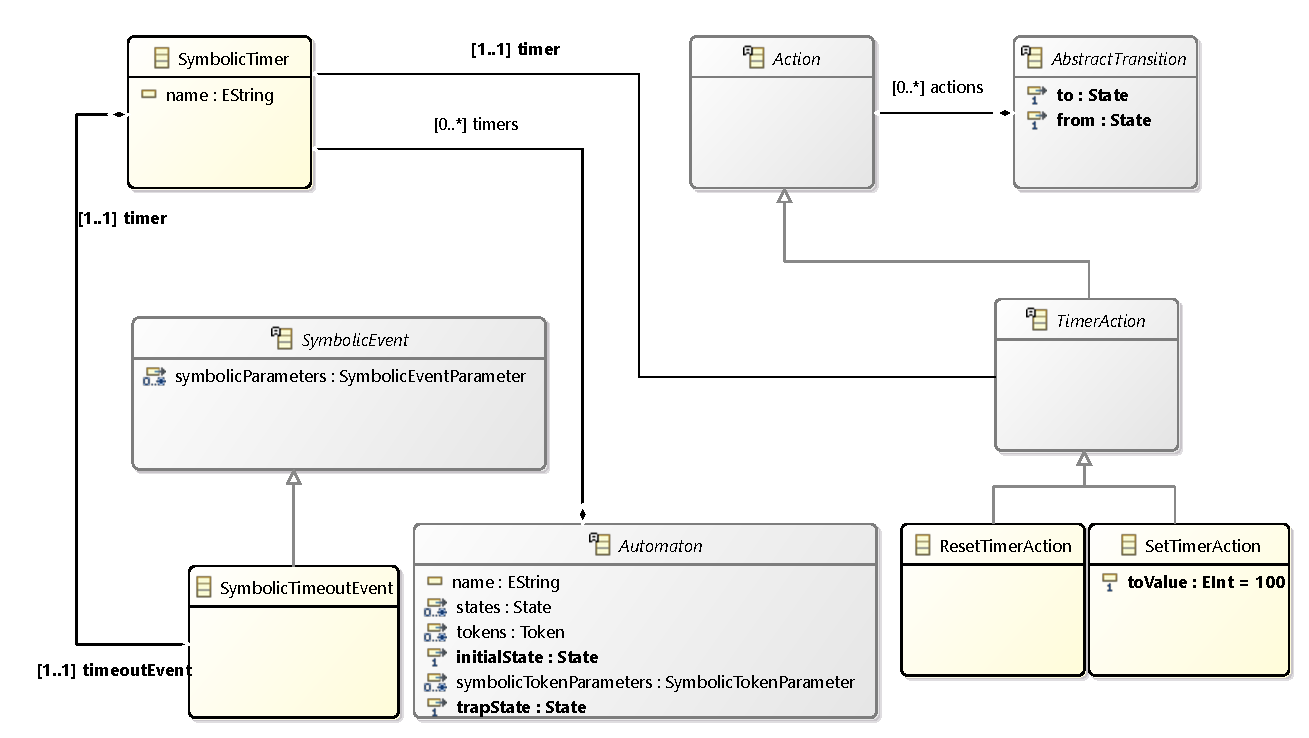
\includegraphics[width=\linewidth]{figures/chapter_5/Timing_diagram}
	\caption{Metamodel of the Timed Event Automaton}
	\label{fig:algo:timed_automaton}
\end{figure}

\subsection{Parameters and Bindings}

The part of the automaton metamodel which is extended with the parametric properties are shown on \cref{fig:algo:parametric_automaton}
The parametrization of the events is represented by the Parameter abstract class. The type of each parameter is implemented with a reference to a SymbolicEvent instance. Parameters can be Fix or Free, an Event only has Fix parameters, but the tokens can have both. Event parameters can be bound to fix values or to a token parameter, this is done by the ConstantBinding and TokenParameterBinding respectively.

\begin{figure}[h]
	\centering
	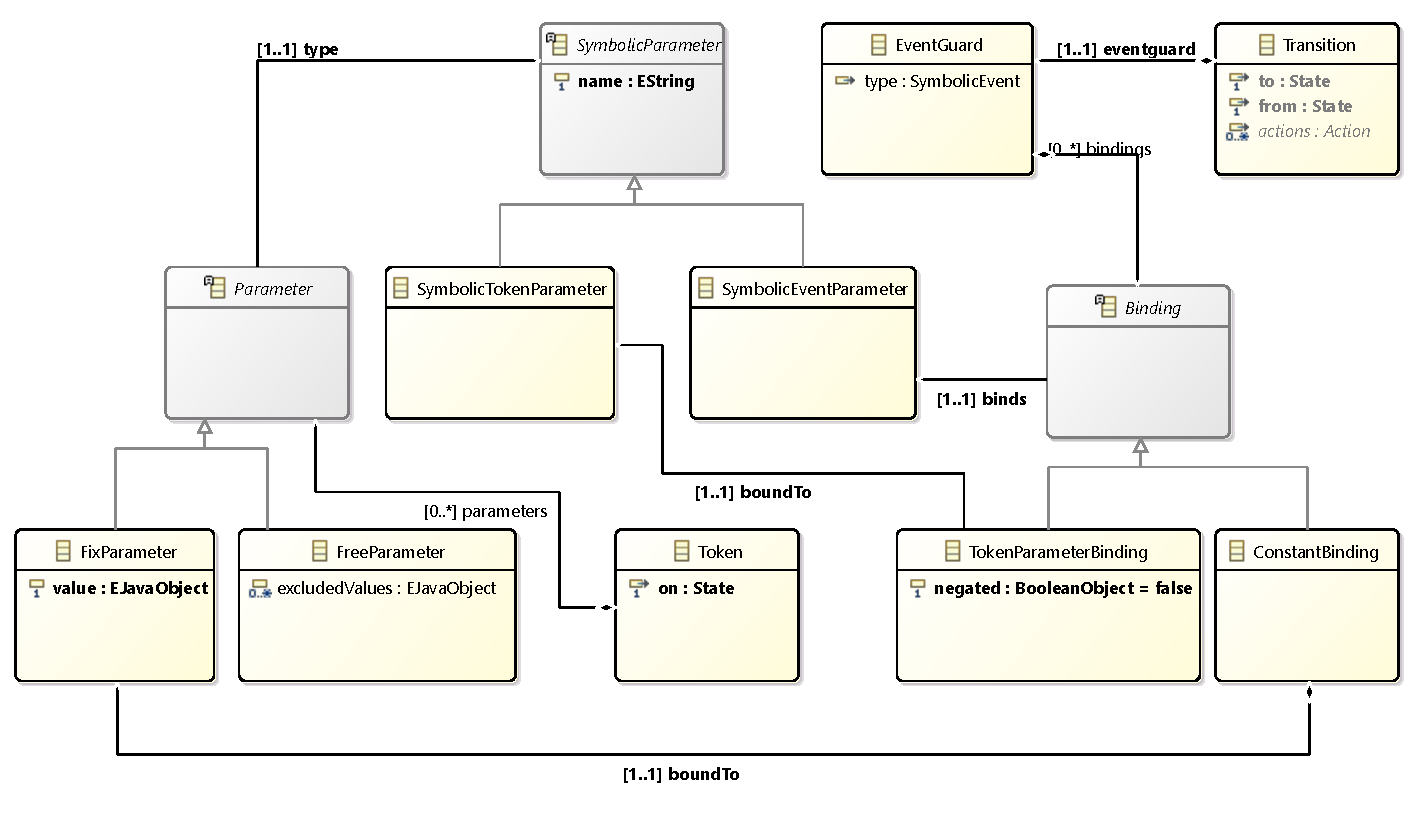
\includegraphics[width=\linewidth]{figures/chapter_5/Parameters_diagram}
	\caption{Metamodel of the Parametric Timed Event Automaton}
	\label{fig:algo:parametric_automaton}
\end{figure}

\subsubsection{Executor}
The algorithm first searches for all the activated transitions.
If it finds an activated transition, it iterates over the tokens which in on that state. The first token with matching (non-confronting)
parameter list will be split to the next state if there are new parameter bindings from the event, or moved if there are no new bindings.
If a token enters an acceptor state it will trigger a function call.

\section{Transformation from VEPL to the intermediate language}


\subsection{VEPL to Regular expressions}
Regular expressions can be built from VEPL patterns, taking the event contexts into consideration
Strict immediate is show on \cref{tab:cep:vepl_regex_strict}, and Chronicle is shown on \cref{tab:cep:vepl_regex_chronicle}.
Each of the patterns must start with a $\Sigma^*$, as in Complex Event Processing every pattern might have arbitrary prefix.


\begin{table}
	\caption{Basic VEPL operators in strict immediate context, expressed with regular expressions}		
	\label{tab:cep:vepl_regex_strict}
	\centering
	\begin{tabularx}{0.5\textwidth}{llX}
		\toprule
		VEPL operator             &	Regular Expression \\
		\midrule
		$p_1$ $\rightarrow$ $p_2$ & $p_1\; p_2$ \\
		$p_1$ OR $p_2$            & $p_1|p_2$ \\
		$p\{\ast\}$               & $p^*$ \\
		$p[t]$                    & $p[t]$ \\ 
		\bottomrule
	\end{tabularx}
\end{table}

\begin{table}
	\caption{Basic VEPL operators in chronicle context, expressed with regular expressions}		
	\label{tab:cep:vepl_regex_chronicle}
	\centering
	\begin{tabularx}{0.5\textwidth}{llX}
		\toprule
		VEPL operator             &	Regular Expression \\
		\midrule
		$p_1$ $\rightarrow$ $p_2$ & $p_1 \; (\Sigma/(p_2))^* \; p_2$ \\
		$p_1$ OR $p_2$            & $p_1|p_2$ \\
		$p\{\ast\}$               & nothing\\
		$p[t]$                    & $p[t]$ \\
		\bottomrule
	\end{tabularx}
\end{table}

\section{Automaton Executor}

	\subsection{Parameter Handling}
	\label{section:algo:paramhandling}

	\subsection{Most Na\"ive approach}
	
	The most na\"ive approach is to keep every potential binding in the memory, for example if there is a pattern $a[i_1]\;b[i_1,\dots,i_n]$ where all parameters are integers and event $a[1]$ happens the state of the memory is shown on \cref{tab:algo:memory}. This indicates that there would be $2^{32^{n-1}}$ objects in the memory, which is not feasible even if $n=3$.\footnote{If each object's size is just 1 bit even then $n=2$ would waste 512MB of memory}
	
	\begin{table}
	\caption{State of the memory on the most na\"ive approach}		
	\label{tab:algo:memory}
	\centering
	\begin{tabular}{ccccc}
		\toprule
		$i_1$ &	$i_2$ & $i_3$ & \dots & $i_n$ \\
		\midrule
		1 	  & 0     & 0     & \dots & 0 \\
		1     & 1     & 0     & \dots & 0 \\
		1     & 0     & 1     & \dots & 0 \\ 
		1     & 1     & 1     & \dots & 0 \\ 
		      &       &\vdots &       &   \\
		1     & 1     & 1     & \dots & 1 \\
		1 	  & 2     & 0     & \dots & 0 \\
		1     & 2     & 1     & \dots & 0 \\
	  	      &       &\vdots &       &   \\
		1     & 2     & 1     & \dots & 1 \\ 
		1     & 2     & 2     & \dots & 0 \\ 
		      &       &\vdots &       &   \\
		1     &$2^{32}$ &$2^{32}$ & \dots & $2^{32}$\\
		\bottomrule
	\end{tabular}
	\end{table}
	
	\subsection{Na\"ive approach}	

	The na\"ive approach is to keep an abstract value for each parameter for each token,
	where the abstract value can be either be
	\begin{itemize}
		\item A concrete value, which shows that for that token the given parameter is bound to that value, i.e.~the given parameter must be exactly that value, or
		\item A list of excluded values which shows that for that token the given parameters values have been reduced by them, i.e.~the given parameter must not be any of the excluded values
	\end{itemize}

	With this approach, every operation seems to be plausible, however a simple counter-example easily shows that the solution is wrong.
	
	Consider the following pattern: $\Sigma^*$ $a[i]$ $\Sigma^*$ $b[i,j]$, i.e.~there must happen an event $a$ with a parameter $i$, and after that there can be any number of events with the functor $b$ with the same first parameter as it was in the first $a$ event. To ease the understanding, the notation will be: The state where the outgoing transition with label $a$ originates will be called $s_0$, the state where the outgoing transition with label $b$ originates will be called $s_1$.
	
	If we would use the na\"ive approach with the input sequence of $a[1]$ $b[1,2]$ $b[1,3]$ the following would happen on reading the inputs one by one:
	\begin{enumerate}
		\item A token would be created on $s_0$ with the binding $i=1$
		\item The token would be split into two, 
	\end{enumerate}

	
	